\chapter{Validation}
Ce chapitre présente les techniques de validation de la plateforme Rsnap. La validation du code est abordée dans un premier temps. Ensuite, les expériences sur des populations d'étudiants et leurs analyses sont développées.

\section{Implémentation}
Dans cette section, les outils de validation du code de Rsnap sont présentés. Deux outils principaux ont été utilisés pour avoir un logiciel le mieux écrit possible \ref{rails-tests} : les tests unitaires et les métriques.

\subsection{Tests unitaires}
Les tests unitaires servent à vérifier que le code fonctionne correctement. L'implémentation des tests s'est déroulée en parallèle à la création de l'application. Deux principaux types de tests ont été réalisés, ceux sur les contrôleurs et ceux au niveau de l'utilisateur. Avant de les aborder, un courte section présente les programmes utilisés pour les tests.

\subsubsection{Outils pour les tests}
Un des programmes utilisés pour les tests est Travis-CI (\ref{travis}). Ce programme est relié à Github pour que tous les tests soient exécutés à chaque commit sur le dépôt. De plus, lors d'une "pull request", les tests sont également effectués pour savoir si l'acceptation de la branche introduira des bogues.

Une des métriques générées par les tests est la couverture du code. Cette information est fournie par Coveralls\ref{biblio} qui est liée à Travis-CI pour l'acquisition des données. Cette métrique est utile pour connaître la fraction du code couvert par les tests. Elle ne donne par contre pas d'information sur le type de code testé. Il faut donc être attentif à ce que les tests couvrent effectivement les parties critiques.

Enfin, lors des tests, il est nécessaire d'avoir des données pour peupler les modèles. Ceci s'effectue grâce au gem FactoryGirls \footnote{\url{https://github.com/thoughtbot/factory_girl_rails}} qui propose un langage dédié pour écrire rapidement des fabriques. Ces dernières vont générer ces données de test pour peupler les modèles.

\subsubsection{Tests au niveau des contrôleurs}
Un premier type de tests est réalisé grâce à RSpec. Ces tests ont pour vocation de vérifier l'accès aux différentes routes \ref{routes} : les droits des utilisateurs et le type de retour des contrôleurs.

Un exemple de test est visible sur dans le code source \ref{lst:rspec}. La partie \texttt{setup} utilise la fabrique spécifique pour créer une mission à chaque test. Deux tests sont ensuite réalisé qui vérifie que seul un utilisateur authentifié peut réaliser une mission.

\begin{figure}
\lstinputlisting[language=Ruby, caption={Test de l'accès au programme associé \`a une mission}, label=lst:rspec]{content/8-validation/validation/program_mission_initializations_controller_test.rb}
\end{figure}

\subsubsection{Tests au niveau de l'utilisateur}
Un deuxième type de tests est réalisé grâce à Cucumber \ref{cucumber}. Ces tests s'effectuent à partir du point de vue de l'utilisateur. Ils assurent le bon fonctionnement des fonctionnalités demandées par l'utilisateur ainsi que des ressources qui en dépendent. Ces tests sont donc de haut niveau, car ce n'est que via les interactions faites sur l'interface que des erreurs internes à l'application peuvent être trouvées.

\begin{figure}
\lstinputlisting[language=Gherkin, caption={Tests de l'accès aux missions}, label=lst:cucumber-mission]{content/8-validation/validation/mission_access.feature}
\end{figure}

\begin{figure}
\lstinputlisting[language=Ruby, linerange={1-15}, caption={Extrait de l'implémentation des tests de l'accès aux missions}, label=lst:cucumber-implementation-mission]{content/8-validation/validation/mission_steps.rb}
\end{figure}

Gerkin est utilisé pour écrire les scénarii en langage naturel. 
Le code source \ref{lst:cucumber-mission} montre différents scénarii décrivant l'accès aux missions. Le haut niveau de Gherkin est visible dans cet exemple. En effet, toute personne anglophone peut comprendre ce que testent les différents scénarii. 

L'extrait de code \ref{lst:cucumber-implementation-mission}, montre comment sont implémentés les scénarii précédents. La façon dont est piloté un navigateur pour réaliser les tests est aussi visible via les méthodes : \texttt{click\_on}, \texttt{current\_path}, \texttt{visit}\ldots

\subsection{Utilisation de metriques}
Un autre style d'outils donne des informations sur le projet via son code source. Deux services ont principalement été utilisés.

\subsubsection{Gemnasium}
Gemnasium \ref{gemnasium} permet d'avoir un service de veille qui vérifie si les dépendances de l'application sont bien à jour et qu'elles ne présentent pas de risque de sécurité.

\subsubsection{rails\_best\_practice}
rails\_best\_practice \ref{rbp} fournit quant à lui une information plus complexe à traiter. En effet, il renseigne les endroits dans le code source qui ne respecteraient pas le "rails way" et en fournit des exemples de réécriture. Cet outil est donc principalement utile en début de projet quand les auteurs ne connaissent pas encore bien quelles sont les bonnes pratiques.

\section{Expériences}
Cette section aborde les expériences réalisées pour ce travail. celles-ci commencent par un après-midi chez KidsCode. Vient ensuite le "Printemps des Sciences" pendant lequel environ 80 élèves ont testé l'application. Enfin, une analyse des expériences à travers des formulaires remplis par les élèves et les professeurs est approchée.

\subsection{KidsCode}
\label{kidscode}
La première expérience s'est déroulée chez KidsCode. Cette organisation a été présentée dans la section \ref{init-kidscode}. C'est une petite initiative locale qui apprend la programmation à 10 enfants âgés de 10 à 14 ans.

\subsubsection{Contexte}
\label{context-kidscode}
Il est important de définir le contexte et la publique de l'expérience qui en influencent considérable son analyse.

Lors de cette expérience, le public était composé de 10 enfants de 10 à 14 ans ayant déjà fait une demi-année de programmation dans le cadre du projet KidsCode. Le niveau de ces enfants n'est donc pas à négliger. Ils sont habitués à exécuter un programme et maîtrisent les principaux concepts de la programmation.

\subsubsection{Buts}
Le but poursuivi dans cette expérience est de valider l'utilisabilité de la plateforme et également le niveau de difficulté des missions proposées. 

Un autre but était de familiariser les expérimentateurs avec des utilisateurs en petit groupe, en vue de préparer la seconde expérience.
Même si ce dernier point pourrait sembler être moins justifié dans le cadre d'un mémoire sur l'informatique, l'aspect pédagogique rentre en ligne de compte dans le cadre de l'utilisation de l'application. Certains paramètres ont pu être identifiés et réfléchis pour leurs implications dans l'expérience ultérieure.
%Pour limiter le plus possible les biais dus à un manque de pédagogie ou d'expérience dans la gestion d'un groupe d'enfant, il était important de pouvoir avoir cette première expérience.

\subsubsection{Déroulement}
L'expérience s'est déroulée pendant un peu plus d'une heure. A la suite des activités habituelles de KidsCode, la dernière heure y était consacrée. 

Le début de l'expérience a été marqué par une perte d'attention et la dissipation des enfants. Une fois le groupe repris en main, les jeunes ont directement montré beaucoup d'intérêts, aussi bien pour l'interface qu'ils découvraient, que pour la compétition intergroupes qui s'est rapidement mis en place.

Comme expliqué dans la partie précédente \ref{context-kidscode}, le public avait déjà de bonnes notions de programmation par rapport au public visé par ce mémoire. Les premières missions ont donc été rapidement réalisées. Les principaux points de ralentissement étaient des problèmes de lecture des consignes. En effet, les auteurs n'avaient prévu que des consignes écrites. Or, les jeunes ne prenaient pas le temps de les lire et ne savaient donc pas quoi faire. Il semble que ce soit l'impatience des jeunes à mener les missions plus que leur niveau de lecture qui détermine leur comportement.

La compétition que les jeunes ont mise en place dès le début a eu un effet bénéfique pour leur évolution car elle leur donnait la motivation de réaliser les défis proposés. Ceci était fort visible à chaque passage de mission. Chaque fois qu'un groupe finissait sa mission, il était important pour lui de le signaler aux autres. Cela lui donnait une satisfaction qui le poussait à réaliser la mission suivante. 

Dans les délais impartis, alors que tous sont arrivés à la mission finale du chien et du chat \ref{chien-chat}, personne n'a réussi à la finir. 

Quand a sonné la fin de l'expérience, beaucoup de jeunes nous ont demandé comment faire pour montrer à leur famille ce qu'ils avaient réalisé et comment faire pour continuer la mission finale.

\subsubsection{Analyse}
\label{analyse-kidscode}
Dans l'ensemble, l'expérience s'est très bien déroulée et les participants ont beaucoup apprécié.

Cependant pour tenir compte de certains paramètres, des améliorations ont été apportées à l'application. Ces modifications sont abordées dans la suite de cette partie.

\paragraph{Changement dans les missions}
La mission \texttt{répète et répépète} a été retirée car elle s'est avérée peu accrocheuse pour les enfants et peu intéressante par rapport aux concepts introduits. Un personnage devait répéter ce que disait un autre. Pendant cette mission, beaucoup d'enfants se sont dispersés parce qu'ils s'embêtaient et que ce n'était pas assez concret. Cette mission avait pour but de faire découvrir les fonctions d'affichage de textes. 

Elle a été remplacée par \texttt{Soyons courtois} décrit en section \ref{mission-courtois}. Cette nouvelle mission est beaucoup plus dynamique que la précédente, car elle permet à l'étudiant de se déplacer et d'utiliseer les capteurs de collisions introduits dans la mission précédente.

\paragraph{Ajout d'un bouton "réinitialiser la mission"}
Lors de l'expérience, un groupe d'enfants a réussi à corrompre l'environnement de la mission suite à une série obscure d'opérations. Pour palier à ce genre de risque, un bouton "réinitialiser la mission" a été rajouté dans l'interface de Snap!. Il permet de réinitialiser la mission courante.

\paragraph{Ajout de vidéo d'introduction}
Comme observé dans cette expérience, les jeunes ont tendance à ne pas lire les textes explicatifs des missions. Il peut en résulter un manque de productivité. Une vidéo d'introduction a donc été rajoutée au début de chaque mission (figure \ref{quelque part}). Cette vidéo explique le but de la mission et donne les instructions. En cas d'oubli, un résumé écrit est toujours présent.

\subsection{Printemps des Sciences}
Cette expérience s'est déroulée dans le cadre de la semaine Scienceinfuse. Des écoles du fondamental et du secondaire viennent participer à des animations dans les universités. L'expérience s'est déroulée avec quatre groupes d'enfants. Ces activités duraient une heure trente y compris les temps d'installation et de prise en charge. Les élèves étaient en programmation par paire \ref{paire} et donc à deux devant un ordinateur.

\subsubsection{Contexte}
Lors de cette expérience, 74 étudiants âgés de 11 à 13 ans étaient répartis en 4 classes, deux de sixième primaire et deux de première humanité.

L'origine des jeunes est également variée. Il y a eu des classes de Chimay, de Bousval et d'Ottignies, ce qui semble être un échantillon suffisamment représentatif.

\subsubsection{Buts}
Le but principal de cette expérience était de confronter l'application à son usage réel dans des classes d'étudiants. Il fallait pouvoir observer comment elle se déroule en réalité et en ressortir une analyse des besoins spécifiques de l'application.

Un autre but poursuivi était l'évaluation de l'âge idéal et du niveau de difficulté des missions pour des néophytes. En effet, lors de l'expérience précédente, le public était volontaire et avait déjà des connaissances en programmation. De par ce fait, le niveau des missions devait être afiné sur le public visé.

Les auteurs désiraient aussi observer les réactions et l'intérêt des étudiants pour la solution proposée.

Un dernier but était évidemment de récolter l'avis des étudiants. 

\subsubsection{Déroulement}
\paragraph{Déroulement général des activités}
Lors de la mise en place de l'activité, une petite démonstration de l'interface a été présentée pour familiariser les étudiants à Snap!. 

Suite à cela, ils ont été invités à créer un compte par groupe de deux (par ordinateur).

Une fois la première vidéo passée, les élèves ont entamé la première mission.\\

La première mission était celle de la voiture, décrite à la section \ref{mission-voiture}. Les étudiants devaient y aborder un concept difficile, à savoir la structuration mentale de leur script. En effet, la voiture revenait à son point de départ à chaque lancement du script. Finalement, après quelques essais et erreurs, ils ont tous réussi cette mission.\\

Une fois la première mission finie, les auteurs ont du rappeler aux étudiants comment la sauver et comment revenir à la liste des missions. Ensuite, les élèves retrouvaient seuls comment continuer. 

Une question récurrente des étudiants était de savoir si leur mission avait bien été enregistrée sur le serveur.\\

À la fin de l'expérience, tous les participants ont reçu un diplôme avec l'adresse web de l'application, afin qu'ils sachent continuer leur programme chez eux.

\paragraph{École Sainte-Marie} 
La première classe à avoir testé l'application est une sixième primaire de l'école Sainte-Marie de Bousval. Le groupe était composé d'une petite vingtaine d'élèves.

L'activité s'est déroulée avec une petite contrariété informatique. En effet, l'interpréteur JavaScript des machines mises à disposition était très lent. Ceci n'a pas compromis le déroulement de l'activité, mais fut, à quelques moments, une source de frustrations pour certains élèves très enthousiastes.

À la fin du temps imparti, tous les élèves avaient atteint la dernière mission, décrit en section \ref{chien-chat}. Ils n'ont généralement pas fini l'étape de déplacement du personnage, mais étaient bien avancés en ce sens.

\paragraph{L'athénée royal Paule Delvaux}
Cette école est venue avec une classe de sixième primaire également. Pour cette expérience, le problème de réactivité de l'interface a été corrigé.

Par rapport a l'école de Bousval, les élèves semblaient avoir moins de facilité à comprendre et moins autonomes.
Cependant, ils sont arrivés à peu près aux mêmes résultats que ceux de Bousval.

L'enthousiasme des jeunes était également au rendez-vous et ils se sont bien amusés.

\paragraph{Collège saint Joseph}
Les deux dernières classes à participer à l'expérience étaient du collège saint Joseph de Chimay accompagnées par leur professeur de mathématique qui semblent induire auprès de leurs élèves un intérêt pour la logique, entre autres de programmation.

Comme ces deux classes avaient un niveau de première humanité, les enfants étaient plus autonomes. L'expérience s'est déroulée comme pour les primaires. La première mission était la plus laborieuse, mais une fois celle-ci passée, le reste a été plus aisé. Ces enfants étant plus grands, il a semblé aux auteurs qu'ils présentaient une capacité d'apprentissage plus élevée. En effet, ils ont été beaucoup plus rapides pour réaliser les missions. Ceci leur a permis d'avancer davantage dans la dernière mission. Certains groupes ont même réaliser un programme fonctionnel pour cette dernière mission: il ne manquait que le score à implémenter.\\

Dans ces classes une différence de niveau au sein des groupe a été observé. En effet certains duos étaient très autonome alors que d'autre se rapprochaient plus des groupes de l'enseignement fondamental.

\subsubsection{Analyse}
\label{analyse-scienceinfuse}
Tout en tenant compte des remarques précédentes, l'ensemble de ces expériences s'est globalement bien déroulée. Les objectifs ont été approchés. Le niveau des missions correspondait à ce qui était souhaité. La plupart des enfants a très vite et bien pris en main l'interface de Snap!. Les modifications apportées par la première expérience ont montré toutes leurs utilités. En autre, le bouton "réinitialisation" s'est avéré facile à utiliser. La mission \texttt{Soyons courtois}, voir section \ref{mission-courtois}, a été appréciée des enfants et a remplis pleinement son rôle.\\

Une crainte était que grâce au lecteur \texttt{YouTube}, ils regardent d'autres vidéos, mais il n'en fût rien et leur curiosité était assez forte pour les garder dans l'application.

Ces expériences ont mis en évidence d'autres améliorations possibles: 
\begin{itemize}
  \item ajouter un message d'information sur la sauvegarde des projets ;
  \item diminuer le taux de rafraîchissement de la fenêtre ;
  \item diviser la mission hélicoptère en deux missions séparées: la boucle "répéter indéfiniment" et la condition "si".
\end{itemize}

Par des expériences ludiques menées en une heure, les enfants ont appris des concepts basiques de la programmation. Les auteurs se sont rendu compte que beaucoup d'enfants n'avaient pas vu le temps passé.

\subsection{Analyse des formulaires}
\label{analyse-exp}
Un formulaire a été complèté par chaque enfants et chaque professeurs à la fin de l'activité. Dans cette partie, les formulaires sont analysés. Les données complètes, les graphiques et les commentaires sont disponibles en annexe, section \ref{annex-data-form}.

\paragraph{Niveau des enfants en informatique}
Une des questions du formulaire portait sur la connaissance de l'informatique et de la programmation. Les schémas montrent comment les enfants auto-évaluent leurs compétences en informatique et en programmation avant de faire l'expérience \ref{fig:niveau-avant} et après l'expérience \ref{fig:niveau-apres}.
\begin{figure}
  \begin{center}
    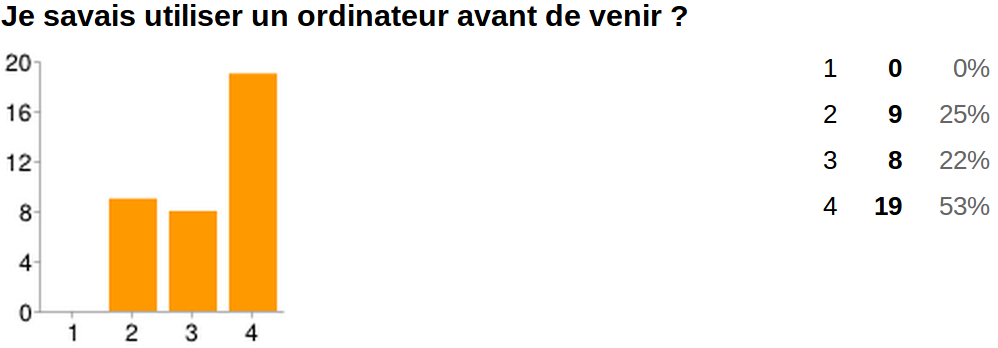
\includegraphics[width=.7\textwidth]{content/8-validation/images/avant}
    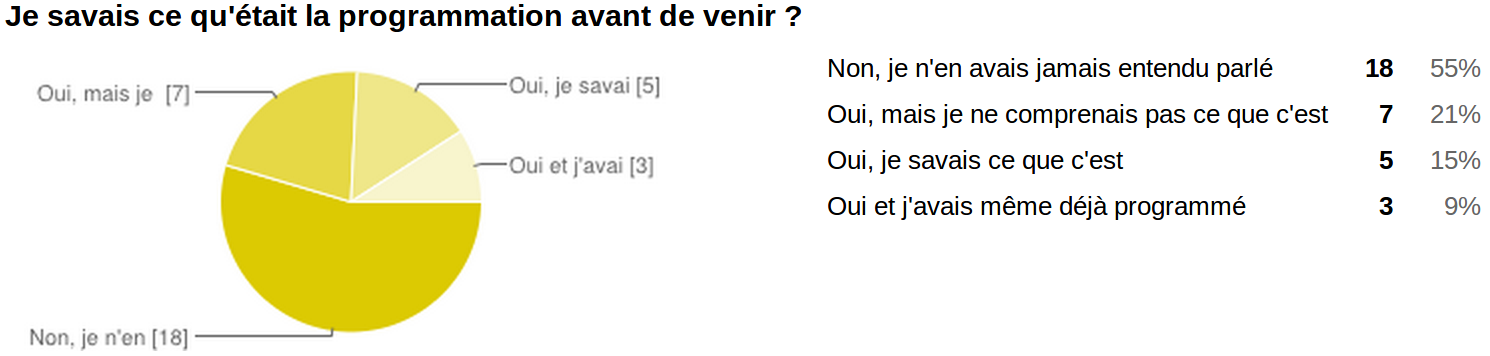
\includegraphics[width=\textwidth]{content/8-validation/images/programmation}
    \caption{Auto-estimation du niveau en informatique et en programmation des participants avant l'activité}
    \label{fig:niveau-avant}
  \end{center}
\end{figure}

\begin{figure}
  \begin{center}
    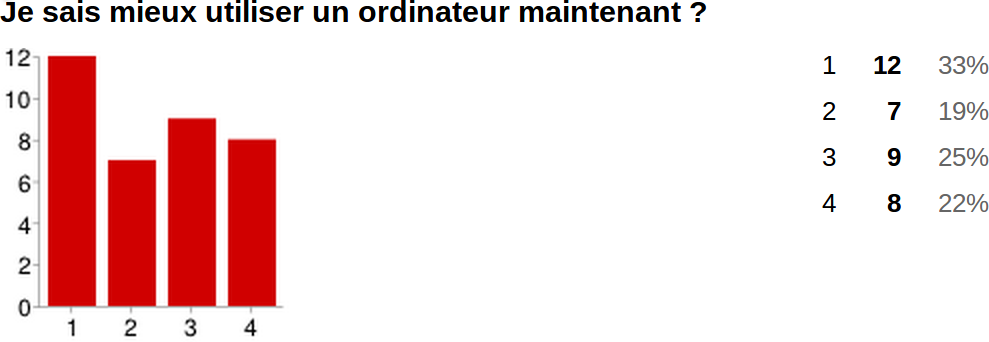
\includegraphics[width=.7\textwidth]{content/8-validation/images/apres}
    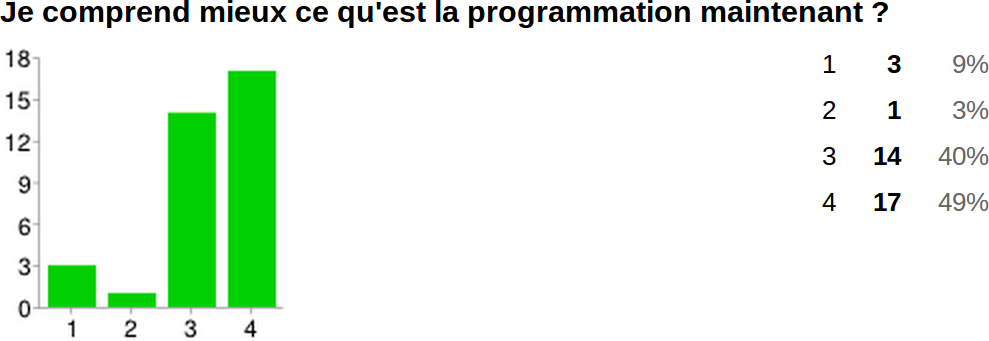
\includegraphics[width=.7\textwidth]{content/8-validation/images/apres-programmation}
    \caption{Auto-estimation du niveau en informatique et en programmation des participants après l'activité}
    \label{fig:niveau-apres}
  \end{center}
\end{figure}

\paragraph{Appréciation des missions}
\label{appreciation}
En plus de l'évaluation de leur niveau de compétences en informatique et en programmation, les participants ont également évalué séparément chaque mission. Les graphiques représentant cette évaluation sont sur la figure \ref{fig:evaluation-mission}. On voit que les missions qui ont été le moins appréciées sont la troisième, "soyons courtois", et la quatrième, "chien et chat".
Sur base des commentaires et de l'appréciation des auteurs, la notation de la quatrième mission peut s'expliquer par la frustration des utilisateurs de ne pas avoir eu le temps de la finir.
Pour la troisième mission, les retours indiquent que les élèves ont trouvé cette mission trop simple. Cette mission pourrait être reconstruite ultérieurement en intégrant, par exemple, le déplacement du personnage.\\


\begin{figure}[ht]
  \begin{center}
    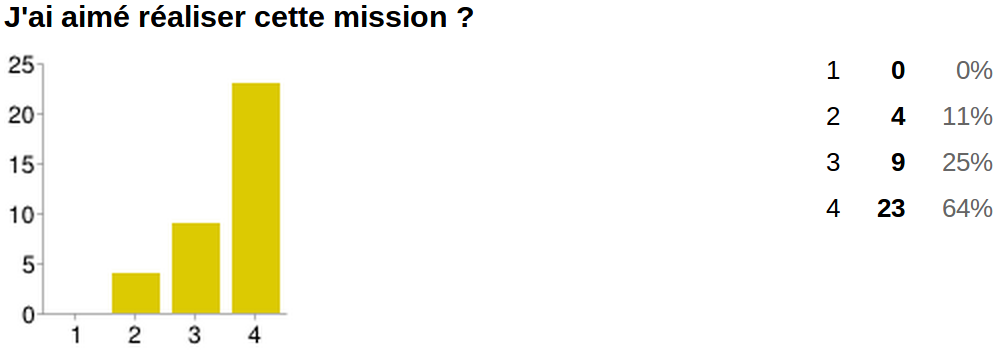
\includegraphics[width=.7\textwidth]{content/8-validation/images/voiture}
    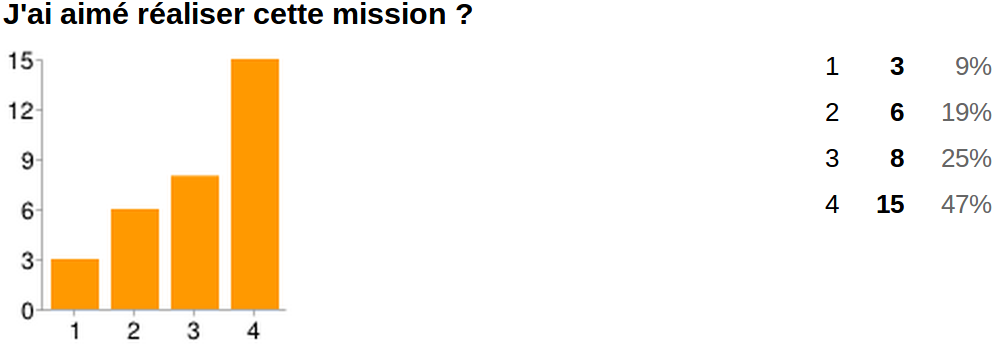
\includegraphics[width=.7\textwidth]{content/8-validation/images/helico}
    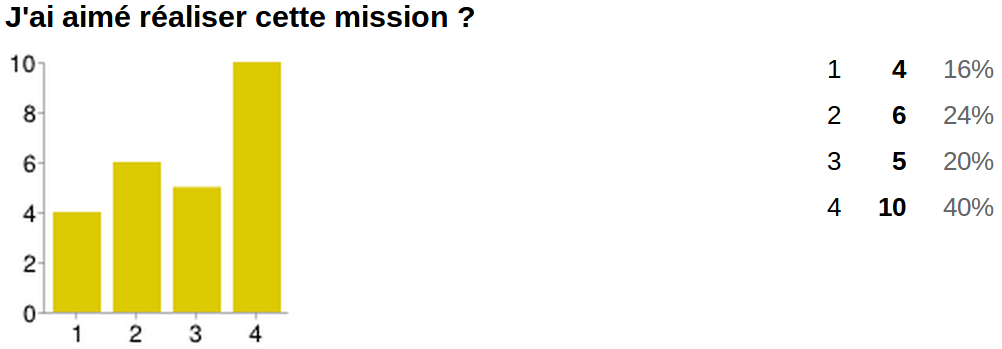
\includegraphics[width=.7\textwidth]{content/8-validation/images/courtois}
    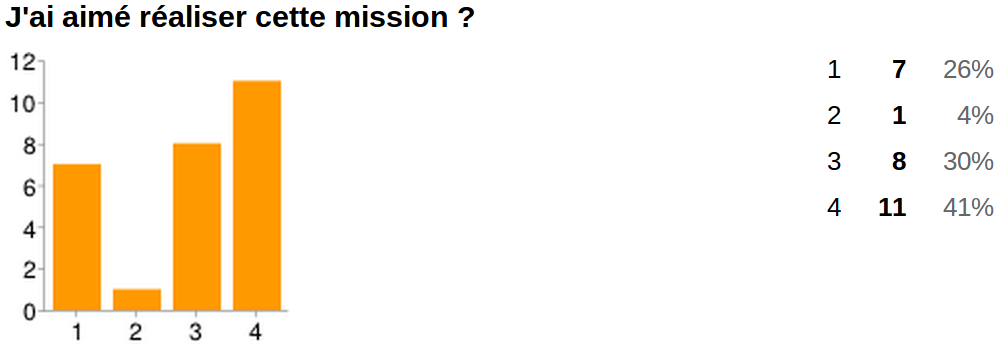
\includegraphics[width=.7\textwidth]{content/8-validation/images/chien}
    \caption{Évaluation des missions par les enfants: En voiture \ref{mission-voiture}, hélicoptère \ref{mission-helicoptere}, soyons courtois \ref{mission-courtois}, tu ne m'attraperas jamais \ref{chien-chat}}
    \label{fig:evaluation-mission}
  \end{center}
\end{figure}

\paragraph{Appréciation des professeurs}
En ce qui concerne les retours des professeurs, voir annexe \ref{result-prof}, ils étaient tous, sans exception, très positifs. Les professeurs d'humanité ont montré beaucoup d'intérêts pour l'utilisation de l'application dans leurs cours. Malgré l'insistance des auteurs, les professeurs n'ont pas donné de critique.

\paragraph{Analyse des missions}
Pour les utilisateurs, la première mission a été la plus laborieuse. Cependant, cette mission a le plus haut taux d'appréciation des enfants. Est-ce du à la facilité de compréhension de cette mission? Est-ce le graphisme? Ou encore son côté concret? Les formulaires n'apportent pas assez d'éléments de réponse.\\

La seconde mission, celle de l'"hélicoptère", a été appréciée, mais, comme cité plus haut \ref{analyse-scienceinfuse}, elle pourrait être séparée en deux missions. En effet, beaucoup d'étudiants ont eu besoin de l'aide des auteurs pour cumuler les deux concepts abordés en une fois.\\

La troisième mission, "soyons courtois", est la moins appréciée. D'après les retours des élèves, elle semble être trop facile. Comme suggéré plus haut \ref{appreciation}, une piste serait de rajouter l'implémentation des mouvements à cette mission.\\

La quatrième mission, "chien et chat", a passionné les élèves mais ils ont été frustrés par le manque de temps. Personne n'a réussi à la finir. Il faudrait peut-être envisager de guider davantage les étudiants dans cette mission. Par exemple, tous les blocs y étaient accessibles, ceci afin que les étudiants puissent découvrir ce qui est possible de faire avec Snap!. L'analyse des questionnaires montre que les étudiants se perdent dans la masse de blocs disponibles.
Une autre possibilité serai d'augmenter le temps imparti à l'expérience tout en tenant compte de la capacité de concentration des enfants. Une durée qui semble intéressante serait deux plages de cinquante minutes.

\paragraph{Tranche d'âge}
\label{trancheage}
Un des objectifs de ce travail est que les enfants utilisent cette application de manière quasi-autonome. Dans ce sens, durant les expériences, les auteurs ont constaté que les enfants de début d'humanité sont plus aptes à travailler de cette manière que les élèves de primaire: moins d'appel à l'aide, plus de persévérance, meilleur prise en charge individuelle, etc.
En conséquence, l'application pour des élèves du fondamental, nécessite soit une plus grande maîtrise de la matière soit plus d'encadrants.

% Les grands vont plus vite

% mission voiture cool pour la structuration
% débouché sur du concret

% différence d'age
% appréciation des missions



%chiffre et analyse de notre formulaire prof et student.
